\documentclass{beamer}
\usetheme{default}
\usepackage{listings}
\usepackage{color}
\usepackage{hyperref}

\definecolor{dkgreen}{rgb}{0,0.6,0}
\definecolor{gray}{rgb}{0.5,0.5,0.5}
\definecolor{mauve}{rgb}{0.58,0,0.82}

\def \lstrset {\lstset{ language=R, basicstyle=\scriptsize,frame=single,
    keywordstyle=\color{blue},stringstyle=\color{mauve},commentstyle=\color{dkgreen}}}

\title{Time series in R}
\author{Andrzej Pragacz}

\begin{document}


\titlepage

\section{Theory}

\begin{frame}{What are time series?}
\begin{itemize}
\item A time series is a sequence of data points, measured typically at successive
points in time spaced at uniform time intervals.
\item Simulation of some random process
\end{itemize}
\end{frame}

\begin{frame}{Applications of time series}
\begin{itemize}
\item signal processing
\item pattern recognition
\item econometrics
\item mathematical finance
\item weather forecasting
\item earthquake prediction
\item electroencephalography
\item control engineering
\item astronomy
\item communications engineering
\end{itemize}
\end{frame}


\begin{frame}{Time series - related packages in R}
\begin{itemize}
\item xts
\item sspir
\item TSA
\item vars
\item tseries
\end{itemize}
\end{frame}

\begin{frame}{White noise}
Identically indepently distributed random variables with normal distribution ($\epsilon_t \sim N(0, \sigma^2)$)

In R 100 samples with distribution $N(0, 1)$ can be obtained in this way:
\lstrset
\lstinputlisting{R/xts/white_noise.R}

\end{frame}


\begin{frame}{Basic time series models}

Moving-average model (MA(q)):
$$
X_t = \mu + \epsilon_t + \Theta_1 \epsilon_{t-1} + \ldots + \Theta_q \epsilon_{t-q}
$$

Autoregressive model (AR(p)):
$$
X_t = c + \epsilon_t + \phi_1 X_{t-1} + \ldots + \phi_p X_{t-p}
$$
Autoregressive moving-average model (ARMA(p,q)):
$$
X_t = c + \epsilon_t + \phi_1 X_{t-1} + \ldots + \phi_p X_{t-p} + \Theta_1 \epsilon_{t-1} + \ldots + \Theta_q \epsilon_{t-q}
$$

\end{frame}

\begin{frame}{Autocovariance \& Autocorrelation}

Autocovariance is covariance applied on time series at given point and shifted self

$$
C_X(t,s) = Cov(X_t, X_s) = E(X_t - \mu_t)(X_s - \mu_s) = E(X_t X_s) - \mu_t \mu_s
$$

For stationary processes, autocovariance simplifies:

$C_X(\tau) = Cov(X_t, X_s) \quad \forall t,s \quad t -s = \tau$

And autocorrelation is normalized autocovariance:

$$
c_x(\tau) = \frac{C_X(\tau)}{\sigma^2}
$$

Where $\mu_t = E(X_t)$, $\mu_s = E(X_s)$, $\sigma_t = Var(X_t)$, $\sigma_s = Var(X_s)$



\end{frame}


\section{The xts package}

\subsection{Basic usage}

\begin{frame}{Loading and plotting time series}
loading:
\lstrset
\lstinputlisting{R/xts/loading.R}

displaying summary, plotting:
\lstrset
\lstinputlisting{R/xts/playing_around.R}
\end{frame}

\begin{frame}{SP500 Plot}
\begin{center}
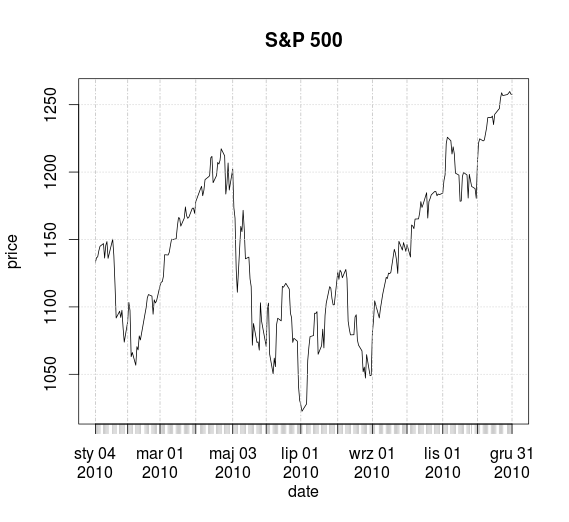
\includegraphics[width=0.8\textwidth]{img/SP500.png}
\end{center}
\end{frame}

\begin{frame}{Processing time series}

Calculating returns:
\lstrset
\lstinputlisting{R/xts/processing_returns.R}

Rolling mean / standard deviation:
\lstrset
\lstinputlisting{R/xts/processing_roll.R}
\end{frame}

\begin{frame}{Returns histogram}
\begin{center}
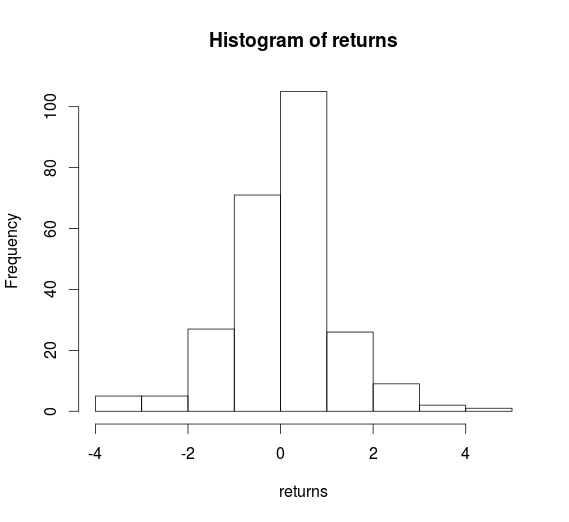
\includegraphics[width=0.8\textwidth]{img/returns_hist.png}
\end{center}
\end{frame}

\begin{frame}{Rolling mean}
\begin{center}
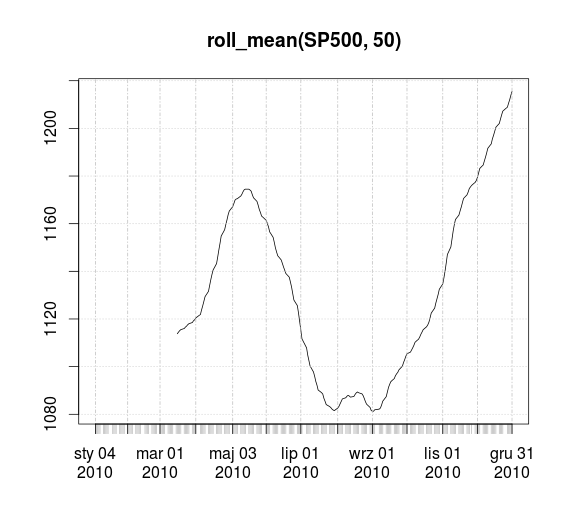
\includegraphics[width=0.8\textwidth]{img/roll_mean.png}
\end{center}
\end{frame}

\begin{frame}{Rolling standard deviation}
\begin{center}
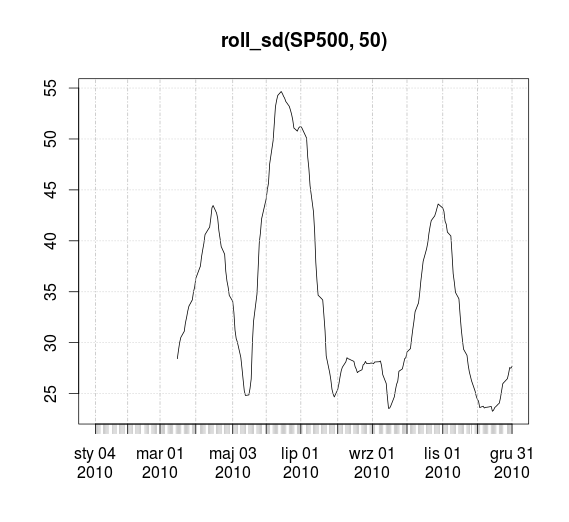
\includegraphics[width=0.8\textwidth]{img/roll_sd.png}
\end{center}
\end{frame}

\subsection{ARMA}

\begin{frame}{ARMA model simulation and estimation}
Simulating the AR(2) process
\lstrset
\lstinputlisting{R/xts/arima_simulate.R}

Estimating the AR(1) coefficients for SP500 example
\lstrset
\lstinputlisting{R/xts/arima_fit.R}

\end{frame}

\subsection{Exponential smoothing}

\begin{frame}{Forecasting using Holt-Winters (exponential smoothing)}

The exponential smoothing formula:
$$
s_0 = x_0
$$
$$
s_t = \alpha x_{t-1} + (1 - \alpha) s_{t-1} \quad \forall t > 0
$$

Using the exponential smoothing for forecasting:
\lstrset
\lstinputlisting{R/xts/holt_winters.R}

\end{frame}


\begin{frame}{Forecasting using Holt-Winters}

\begin{center}
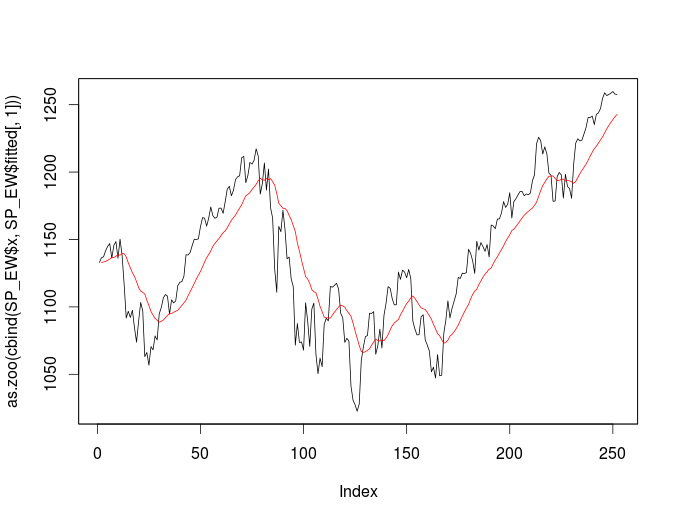
\includegraphics[width=0.8\textwidth]{img/holt_winters.png}
\end{center}

\end{frame}

\subsection{Lag operator}

\begin{frame}{Lag operator}

Following notation is used:
$$
L X_t = X_{t-1}
$$
Other way of describing AR(p) model:
$$
\epsilon_t = (1 - \sum_{i=1}^{p} \phi_i L^i) X_t
$$

\lstrset
\lstinputlisting{R/xts/lag_operator.R}

\end{frame}

\section{The sspir package}

\subsection{Kalman filter}

\begin{frame}{Kalman filter}

\lstrset
\lstinputlisting{R/sspir/kalman_filter.R}

\end{frame}

\begin{frame}{Kalman filter}

\begin{center}
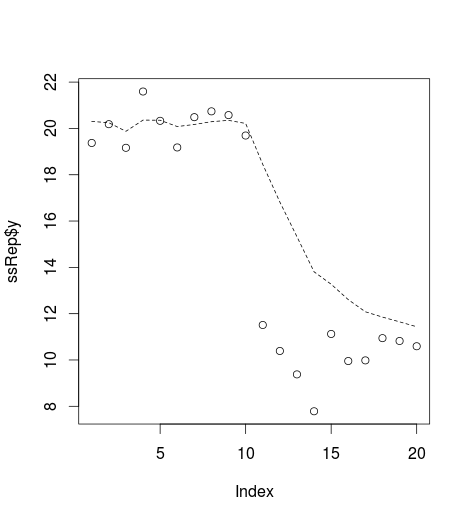
\includegraphics[width=0.6\textwidth]{img/kalman_filter.png}
\end{center}

\end{frame}

\section{The TSA package}

\subsection{Periodogram}

\begin{frame}{Plot of y}

\begin{center}
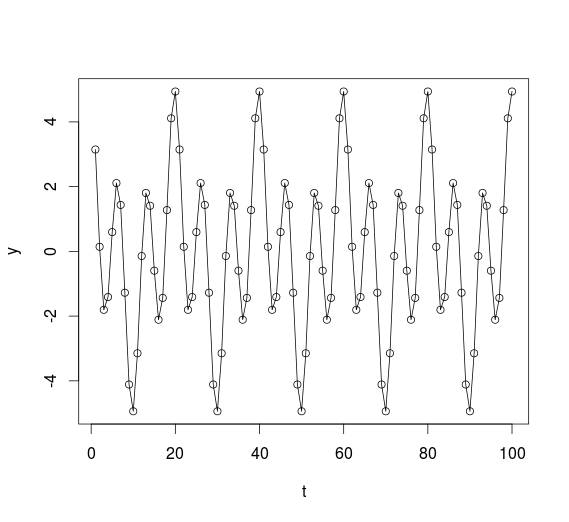
\includegraphics[width=0.8\textwidth]{img/cos_y.png}
\end{center}

\end{frame}

\begin{frame}{Periodogram of y}

\begin{center}
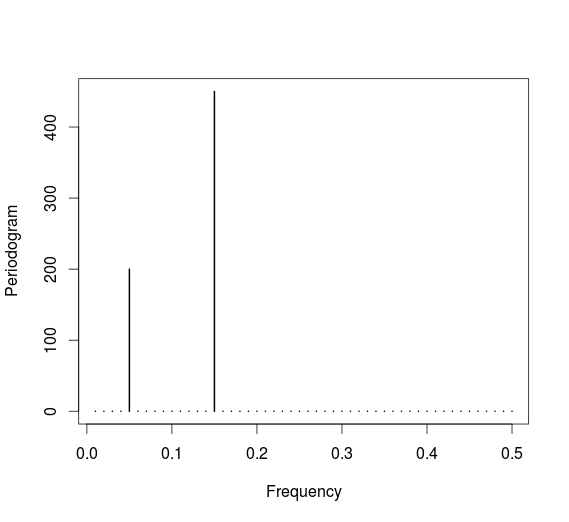
\includegraphics[width=0.8\textwidth]{img/cos_y_periodogram.png}
\end{center}

\end{frame}

\section{Other topics}


\begin{frame}{Other topics not mentioned here}
\begin{itemize}
\item Vector Autoregression
\item Cointegration
\item Granger causality
\end{itemize}
\end{frame}

\begin{frame}
Questions?
\end{frame}

\end{document}
